\chapter{Analysis}\label{ch:analysis}

\summary{
We have now devised a fully-fledged document layout system that works across many platforms. In this chapter we discuss the layouts produced by the system both quantitatively and qualitatively, and put the system to the test in a user study.
}

%\section{View-time Operations}

\section{Quantitative}

Chapter~\ref{ch:intro} (and in particular Section~\ref{sec:goodtypesetting}) provides an overview of some of the operations required when laying out a document. This section examines this in further depth, and contrasts the operations required to view fixed and flowable documents against the operations required to view malleable documents.

\subsection{Fixed Document Formats}
Documents in a fixed format are rendered in a manner similar to the following:
{\singlespacing
\begin{lstlisting}
parse and tokenise the document layout instructions;
foreach (layout instruction) {
    interpret and execute the instruction;
}
paint the results to the screen;
\end{lstlisting}
}
With the notable exception of PostScript, which is Turing complete, the majority of fixed document formats have only declarative layout instructions, and do not permit computation. This helps ensure that the document is always rendered identically.\hspace{0pt}\cite{Bagley2007}

\newpage
\subsection{Flowable Document Formats}

When a document in a flowable format is to be laid out, the process is as follows:
{\singlespacing
\begin{lstlisting}
parse the source to identify flowable blocks;
foreach (flowable block) {
    apply a line-breaking algorithm;
}
paint the results to the screen;
\end{lstlisting}
}

This process generates information similar to that contained in fixed-format documents, which is then used to drive the painting of contents to the screen.

The line breaking algorithm can be as simple as or complex as desired. In most cases, the line-breaking algorithm used by flowable documents is reasonably simple, and will take a first fit approach. This will be of the form:

{\singlespacing
\begin{lstlisting}
parse block to identify all possible breakpoints;
while (non-breakable items remain to be laid out) {
    place one item on the current line;
    if (there is not space for the next item) {
        adjust spacing between items to justify;
        move to a new line;
    }
}
\end{lstlisting}
}

As is noted in Section~\ref{sec:goodtypesetting}, first-fit algorithms do not generally result in well-typeset output. The simplest of these algorithms will not attempt to identify potential hyphenation points. More complex layout algorithms that search for ``optimal'' layouts usually require a considerable amount of backtracking and are thus more computationally demanding.

\newpage
\subsection{Malleable Documents}

The layout algorithm for a malleable document is as follows. First, the penalties are calculated:

{\singlespacing
\begin{lstlisting}
foreach (included galley rendering) {
    compute penalty for the rendering at current page width;
}
select the rendering with the minimum penalty;
\end{lstlisting}
}


Then, using the galley rendering that has the lowest penalty, the content is laid out onto the screen:

{\singlespacing
\begin{lstlisting}
foreach (paragraph-level item in selected galley rendering) {
    foreach (line-level item in paragraph) {
        use precomputed data to place words;
    }
}
paint the results to the screen;
\end{lstlisting}
}
Crucially, a number of complex steps have been moved from view-time to compile-time (as they are for fixed-format documents) but without flowability being sacrificed:
\begin{itemize}
 \item The source is already parsed into a form optimised for layout
 \item The line-breaking has been entirely precomputed
\end{itemize}
One step has been added: each included galley rendering must be examined once before layout, in order to ascertain its ``penalty'' for use. The penalty is based entirely on the width of the page, and the \gls{measure} (width) of the galley rendering.%, and is described in more detail in Section~\ref{sec:layout}.

This penalty is calculated by taking the extra required horizontal whitespace (which can be envisaged as slack between columns) and weighting this to further penalise large numbers of columns. This weighting is achieved by multiplying by a smaller-than-linear function of the number of columns, such as a square root or logarithm.

Many low-power processors do not come with floating-point hardware as standard (for example the \textsc{arm} range of processors) which might suggest that these are poor choices of functions since they must be emulated using integer and bitwise operations only. This is not particularly important, for a number of reasons. Firstly, it has been shown previously\hspace{0pt}\cite{Lomont2003} that it is often possible to use mathematical analysis to find extremely good approximations for such functions. Secondly, the range of inputs to such a function would be limited to integers ranging from 1 to (in an extreme case) about 20, so the values could be pre-computed and stored in a lookup table. Thirdly, the penalty (and hence the root or logarithm) is calculated precisely once for each included galley rendering: in Sections \ref{sec:inc-renderings}~and~\ref{sec:survey} it is suggested that between three and ten galley renderings should be included in any one document. Given these facts, it is clear that there will be little impact from using such a function in the penalty calculation. In any case, as Don Knuth famously (and perhaps a little overdramatically) stated: ``\emph{premature optimization is the root of all evil}''.\hspace{0pt}\cite{Knuth1974}


Most importantly, since the line-breaking algorithm has been moved to compile-time, there is no longer any requirement to limit its complexity. In fact, should the need (or desire) arise, the text layout can be hand-tuned, or \emph{entirely hand-typeset}, with no consequences at view-time.


\subsection{Handling of Floats}
\label{sec:quant-floats}

The grid-based layout system devised in Section~\ref{sec:gridlayout} works in a similar manner to a first-fit line-breaking algorithm, in that it places elements on the page in order, in the first place they will fit. In the case of this system, each element is a floatable figure or line of text. Elements that are the same size as a single grid cell, such as lines of text set in the main point size, can simply be placed in the first empty slot in the current column, or the first empty slot in the next column, should there be no empty spaces.  For the placement of elements that are larger than a single grid cell, there is some overhead required to step through the grid until a suitable position can be found. Once a position has been found, each grid cell that it overlaps must be marked as being reserved.

In the worst case, this algorithm does have a greater-than-linear time complexity. In practice, so long as the number of floats does not become excessive (which would cause the grid to be walked many times to search for suitably large gaps) the algorithm runs in linear time.

The placement of floats is subject to certain constraints: they must span integer multiples of columns, and can only be placed aligned to grid cells. This is very different to the model used for floats in \gls{html}, whereby floats may be positioned arbitrarily, and text flowed around them. The result of this imposed ``restrictiveness'' on float placement (in comparison with that of \gls{html}) is that the produced layouts are more regular. Each produced document as a whole fits together much better, as we shall see in Section~\ref{sec:aesthetic-quality}.


\newpage

\section{Qualitative}
\label{sec:aesthetics}

\subsection{Placement of Floats}
Since all text layout is precomputed, the only remaining concern is that the columns of text and floats are laid out in a pleasing manner.

Plass\hspace{0pt}\cite{Plass1981} devised a system to perform optimal placement of floats within text, whereby float placement is penalised by the square of the distance from its intended position. He showed that this problem was NP-hard, but he also showed that a similar (but less ``optimal'') system using linear penalties could be made computationally tractable.

Br\"uggemann-Klein et al.\hspace{0pt}\cite{Bruggemann-Klein1995} suggested that Plass's method is only optimal if one agrees with Plass's definition of ``optimal''. They proposed that a superior metric for float placement is to minimise the number of page turns that a reader must perform when reading the document from front to back. This is a desirable characteristic for a pagination algorithm that runs on an \ebook{} reader, because page turns tend to be slow, particularly on devices with electronic paper displays. Unfortunately, the algorithm used runs in quadratic time, which limits its usefulness to this system.

In essence, the assumption that Plass's float placement algorithm produces the most optimal layouts may be slightly short-sighted: \emph{other pagination schemes are available!} Clearly, using computationally complex algorithms such as those devised by Plass and Br\"uggemann-Klein et al. will have a significant impact on the demand for computation at view-time. As with many facets of the system described in this thesis, the float placement algorithm was chosen with efficiency in mind.

The float placement algorithm that has been developed for use with the malleable document system also aims to minimise the distance between the actual and intended positioning of floats: if a float can be placed directly at its intended position, then it will be, otherwise it will be placed in the next available space. (Figure~\ref{fig:floatlayout} on page~\pageref{fig:floatlayout} demonstrates this process.)

Whilst this algorithm does not perform any lookahead or backtracking in order to place floats optimally, anecdotal evidence gained from using the system has shown that in most cases floats are placed directly in their intended position, or at the top of an adjacent column, and are rarely moved across page boundaries. Appendix~\ref{app:layouts} showcases some examples of layouts produced using this algorithm, alongside some comparative renderings of the same document, rendered in \LaTeX{} and \html{}. The output of the malleable document system looks very similar to that of \LaTeX, and very different from that of the web browser.

As it stands, the algorithm does not avoid widowed or orphaned lines, nor single lines directly before or after floats. This can be seen clearly in the example in Appendix~\ref{app:layout-ff} on the e-reader example (page~\pageref{app:p:layout-ff-ereader}) at the top of the fourth page, where the float has spanned both columns and taken up all the space on the page, with the exception of one line at the top of each column. It would be simple to add a constraint that states that single lines of text at the top or bottom of the page must never be allowed, which could be enforced by leaving extra lines blank and pushing the text forward, though it is possible that this may harm the balance of the page if it causes columns to have uneven lengths.


\subsection{Measures of Aesthetic Quality}
\label{sec:aesthetic-quality}
In their 2004 paper, Harrington et al.\hspace{0pt}\cite{Harrington2004} identified a number of aesthetic properties against which automated document layout systems may be measured. Many of these properties are inherently well satisfied by this system, due to its use of a grid to provide regular layout:

\paragraph{Alignment} This property states that all content objects must have some commonality of alignment, based on their edges and/or centreline. Aligning content objects to a grid enforces this.

\paragraph{Regularity} This property states that alignment positions must be regularly spaced\ed an inherent property of a grid.

\paragraph{Balance} This property states that a page's visual weighting should ideally be around the centre of the page, and also that the page must be well balanced between left and right. Since the malleable document system produces pages with uniform density\ed there are no gaps left until the content has all been laid out\ed this property is well satisfied.

\paragraph{Whitespace Free-flow} This property states that whitespace should always be connected to the margins, and that there should never be islands of whitespace. The grid-based columnar layouts produced by the malleable document system ensure that any non-margin whitespace (for example the gaps between paragraphs or before and after floats) is always directly connected to the margin whitespace.

\paragraph{Uniformity} This property states that the visual density of the page should be consistent, \ie{} that content objects should be distributed uniformly. The combination of the above measures (alignment, regularity, balance, and whitespace free-flow) mean that the page's visual density is inherently uniform.

\vspace{2em}
Examining the grid layout float placement algorithm specified in Section~\ref{sec:gridlayout} (in conjunction with the sample layouts shown in Appendix~\ref{app:layouts}) it can clearly be observed that all these characteristic properties are fulfilled by the malleable document system.

\newpage
\section{User Study}
\label{sec:survey}
In order to establish the most appropriate range of galleys to include in a malleable document, as discussed in Section~\ref{sec:inc-renderings}, a user study was conducted. This was also used as a chance to get some general feedback about the malleable document system from a large pool of real-world users.

\subsection{Participants}
The study was carried out entirely online. Participants were recruited via email circulated around the researchers mailing list at the School of Computer Science, and via a number of posts on the web. No personal data was collected from any participants, though due to the recruitment method, it is a reasonable assumption to make that the majority of the participants had prior experience in reading electronic documents on a screen. In all, the study had 41 participants.

\subsection{Methodology}
Obtaining data that can be interpreted quantitatively from a process that is inherently qualitative can be a challenge. It can be difficult to turn \emph{How good did you think this was?} and \emph{Which one of these is better?} into something from which statistical significance can be taken. With enough respondents and the use of some cunning, this can certainly be achieved.

In this user study, each participant was given a malleable document to read, and then asked for their feedback. Each participant was randomly assigned into one of six groups, labelled from A to F. Participants were not made aware that they had been assigned to a group. Each group was presented with a separate instance of a malleable document. These all had the same textual and graphical content, but contained different ranges of galley renderings.

As mentioned in Section~\ref{sec:inc-renderings}, according a consensus among professional typographers is that lines of text should not normally be less than 30 characters wide, nor wider than 75, and that 40--50 characters is reasonable for multi-column work. The pool of galley widths from which each malleable document instance's included renderings were chosen is shown in Table~\ref{tab:galleypool}. These were chosen to extend slightly beyond this range, whilst providing good coverage across it. The table also shows which of these renderings was included in each group's document.

\begin{table}
\begin{center}
\begin{tabular}{rcccccccccc}
\toprule
inches&1.5&2.0&2.5&3.0&3.5&4.0&4.5&5.0&5.5&6.0 \\
characters&22&28&35&42&49&56&63&70&77&84\\
\midrule
A\hspace{1em}$315$~\textsc{kb}& \checkmark & \checkmark & & \checkmark \\
B\hspace{1em}$392$~\textsc{kb}& \checkmark & \checkmark & & \checkmark & & \checkmark \\
C\hspace{1em}$538$~\textsc{kb}& \checkmark & \checkmark & & \checkmark & & \checkmark & & \checkmark & & \checkmark \\
D\hspace{1em}$549$~\textsc{kb}& \checkmark & \checkmark & \checkmark & \checkmark & \checkmark & \checkmark \\
E\hspace{1em}$839$~\textsc{kb}& \checkmark & \checkmark & \checkmark & \checkmark & \checkmark & \checkmark & \checkmark & \checkmark & \checkmark & \checkmark \\
F\hspace{1em}$386$~\textsc{kb}& \checkmark & \checkmark & & & & \checkmark & & & & \checkmark \\
\bottomrule
\end{tabular}
\end{center}
\caption[Galley widths used in documents in the user study]{This table shows both the pool of galley widths that were used in the generation of malleable document instances A--F, which renderings each instance contained, and the filesize of each instance. The number of characters corresponding to the width in inches has been taken from a lookup table in \emph{The Elements of Typographic Style}\hspace{0pt}\cite{Bringhurst2008}. These values are for 12 point Times Roman.}
\label{tab:galleypool}
\end{table}

All documents contained the narrowest two galley renderings. This was to ensure that it would be possible to display the document on an extremely narrow screen and/or with a high scaling factor.

Document A was deliberately designed to provide a poor user experience. It had only three galleys, and only one of these was within the range specified above. Documents B and D both contained galleys up to 56 characters in width, and documents C, E and F contained galleys up to 84 characters in width. Documents B and C contained a coarser range of galleys (and hence fewer) than documents D and E. Document F contained the coarsest range of galleys. These ranges and coarsenesses were chosen in order to assess how their changes affect perceived user experience.


\subsection{Preamble}
At the start of the study, each user was presented with the following:
\begin{verbatim}
 This study is designed to evaluate a variety of document
 layouts, and the way these layouts are interacted with by
 users. You will be asked to read a short document with a
 particular layout, and then fill in a questionnaire about
 your reading experience. Don't worry, this is not a
 comprehension exercise! You may use any device with a
 modern web browser (eg desktop, laptop, tablet, mobile
 phone) though it is preferable that you use a mobile phone
 or tablet, since this is primarily aimed at portable
 devices with small screens. For this reason, if you're
 using a laptop or desktop, you may find it helpful if your
 web browser window is not maximised.

 Very shortly, you'll be given some text to read (taken from
 the Wikipedia article on The Great Fire of London) that
 will be customised to fit the screen you're reading it on.
 Feel free to try changing your browser window size (or
 screen orientation if you're using a phone or tablet). If
 you don't want to read the whole document, it's fine to
 stop once you feel you have looked through it enough to be
 able to answer some questions on the document's layout.

 Before you begin, here are some quick instructions:

 If you're using a laptop/desktop computer with a keyboard:
  *  Use the up/down arrow keys to increase/decrease
     the font size
  *  Use the right/left arrow keys to turn to the
     next/previous page

 If you're using a device with a touchscreen (phone/tablet
 etc):
  *  Swipe up/down on the screen to decrease/increase the
     font size
  *  Swipe left/right turn to the next/previous page
\end{verbatim}



\subsection{Questions}
\label{sec:surveyqs}
Once each user had read the preamble, and had had enough of reading about The Great Fire of London, they were asked for their feedback in the following manner:

\begin{verbatim}
 Please rate the following statements based on how closely
 you agree or disagree with them. For each, choose a number
 from 0 to 10, where 0 is "I strongly disagree", 5 is
 neutral, and 10 is "I strongly agree".

 Q1. The document layouts produced were well-adapted to fit
     my screen.

 Q2. I could adequately customise the document layout to
     suit my personal reading preferences.

 Q3. I would preferentially choose a document layout system
     like this to read long text-based web pages.

 Q4. I would preferentially choose a document layout system
     like this to read PDFs.

 Q5. I would preferentially choose a document layout system
     like this to read ebooks.
\end{verbatim}

Questions 1 and 2 were designed to assess overall impressions of the system, and questions 3--5 to ascertain whether users would feel comfortable using a similar system to read documents in different contexts.
Participants were also given the opportunity to provide written feedback.

\subsection{Discussion of Results}
Table~\ref{tab:sampledocs} and Figure~\ref{fig:surveygraph} show the aggregated response data for each group. It is clear that, especially for questions 1 and 2, renderings D and E are by far and away the most consistently highly rated. These were the two documents that had the least coarse range of galley renderings, which suggests that, as seems intuitive, the inclusion of a greater number of galley renderings within a given range provides a better user experience. It is also clear that the smaller maximum galley width used in rendering D has not had a vast adverse affect on its user rating.

As shown in Table~\ref{tab:galleypool}, rendering D's filesize is approximately 65\% of that of rendering E. Figure~\ref{fig:fsgraph} shows the filesizes of each rendering plotted against their mean scores for questions 1 and 2. This quite neatly illustrates each rendering's tradeoff between filesize and perceived quality, and it is easy to identify that rendering D here makes the tradeoff work best.

As to questions 3, 4, and 5 (``\emph{I would use this for \emph{\{}web pages, PDFs, \ebook s\emph{\}}}'') there does not seem to be much consensus between any of the renderings. Averaging over all responses, the results are web pages:~5.8, \glspl{pdf}:~6.7, and \ebook s:~6.9. This does show a weak preference for the malleable document system for all three, with a stronger preference for \glspl{pdf} and \ebook s.


\begin{table}
  \footnotesize
  \myfloatalign
  \begin{tabular}{cccrcccccc}
    \toprule
    group & range & step & n & respondents & q1 & q2 & q3 & q4 & q5 \\
	& (inches) & (inches) \\
    \midrule
    A & $1.5$,~~$2-3$ & $1.0$ & $3$  & $9$ & $6.8$ & $6.3$ & $5.7$ & $7.1$ & $6.8$ \\
    B & $1.5$,~~$2-4$ & $1.0$ & $4$  & $6$ & $7.7$ & $6.7$ & $6.0$ & $6.3$ & $5.8$ \\
    C & $1.5$,~~$2-6$ & $1.0$ & $6$  & $8$ & $7.1$ & $6.6$ & $4.5$ & $6.0$ & $5.8$ \\
    D & $1.5$,~~$2-4$ & $0.5$ & $6$  & $7$ & $8.1$ & $7.7$ & $5.9$ & $5.9$ & $7.4$ \\
    E & $1.5$,~~$2-6$ & $0.5$ & $10$ & $5$ & $8.6$ & $8.0$ & $8.6$ & $8.0$ & $8.4$ \\
    F & $1.5$,~~$2-6$ & $2.0$ & $4$  & $6$ & $6.5$ & $7.2$ & $5.3$ & $7.0$ & $8.0$ \\
    \bottomrule
\end{tabular}
  \caption[Summary of user study results]{A summary of the data obtained from the user study. For each group A--F, the included renderings are shown (columns \emph{range}, \emph{step} and \emph{n}, respectively the narrowest and widest galleys, the size of steps between them, and the total number of included galleys). The mean value of the responses for questions 1--5 (detailed in Section~\ref{sec:surveyqs}) is shown for each group. Figure~\ref{fig:surveygraph} shows a plot of this data in greater detail.}
  \label{tab:sampledocs}
\end{table}

\begin{sidewaysfigure}
  \begin{center}
  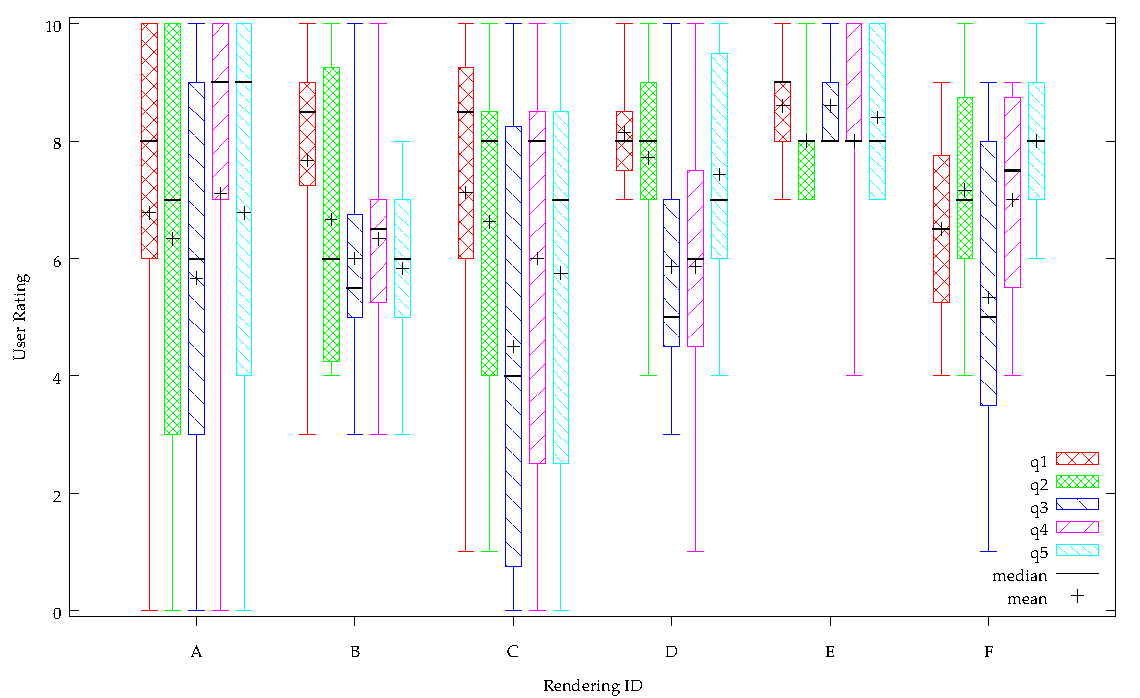
\includegraphics[height=0.5\textheight]{gnuplot/survey.pdf}
  \end{center}
  \caption[Plot showing user study results]{This plot shows the distributions of responses to each survey question for each group of respondents. The boxes mark the interquartile ranges, and the whiskers show the full range. The mean and median values are also shown (as indicated in the key). Questions 1 and 2 are of the most import: respectively, these assess whether the user thought the layouts fitted well to their screen, and whether the user thought they could customise the layout to suit their reading preferences.}
  \label{fig:surveygraph}
\end{sidewaysfigure}

\begin{sidewaysfigure}
  \begin{center}
  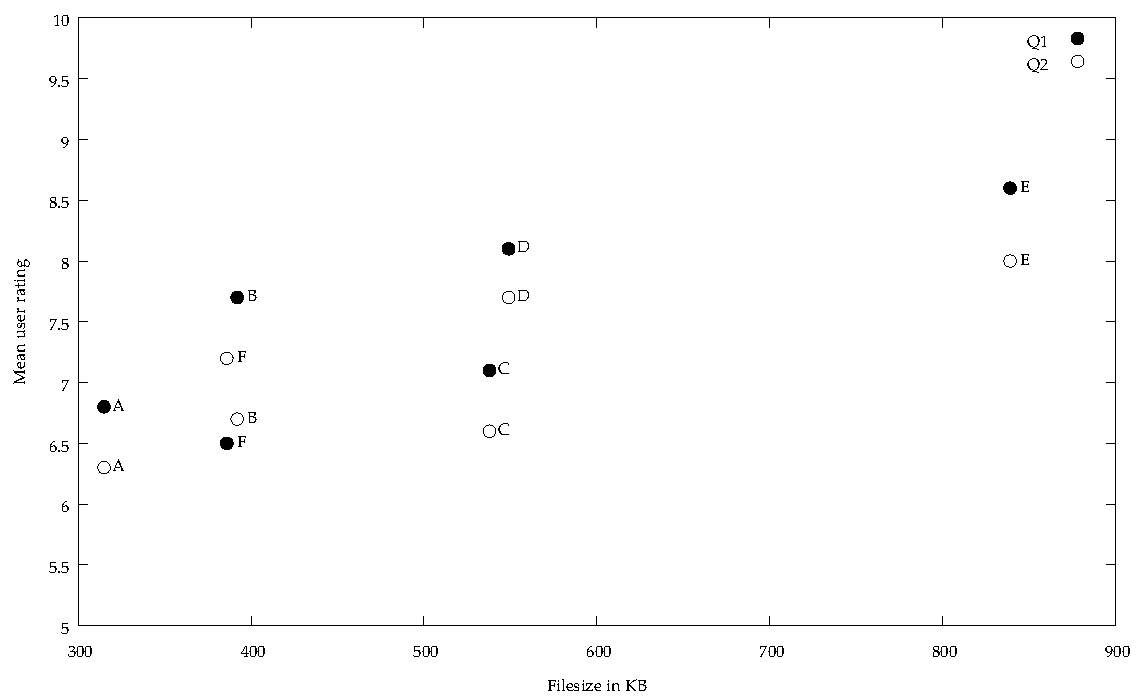
\includegraphics[height=0.5\textheight]{gnuplot/fsizes.pdf}
  \end{center}
  \caption[Plot of user rating against filesize]{This plot shows the mean of each group's responses to questions 1 and 2 against the filesize of that group's document. Although group E scored highest, group D's scores are not far behind, and its filesize is some 65\% of group E's.}
  \label{fig:fsgraph}
\end{sidewaysfigure}

\subsection{User Comments}
Some comments from users follow:

{\raggedright
\begin{quote}
``Initially the unconventional method of adjusting the type size by swiping vertically seemed out of place and a little jarring when it is standard practice to swipe vertically to scroll webpages etc on an iPhone - swiping to turn pages, typically reserved for ebooks does work well in this application of the gesture. However, without the instructional prompt before reading the article I would have probably taken some extra attempts to realise swiping ebook-style would progress through the article. The way the text flowed into columns etc while adjusting the size was fluid and ensured any preference could easily be achieved. Overall I liked the way it worked.''
\end{quote}

\begin{quote}
``The thing that put me off the viewer most was the fact that it enforced a page model on a continuous flow document and in so doing broke the browser's native scroll ability. This meant that I couldn't use the mouse wheel to scroll, and I couldn't jump to arbitrary points in the document using the scrollbar. I would have much preferred a single continuous column that my browser could scroll through normally, and this is also true if I were browsing on a mobile device.''
\end{quote}

\begin{quote}
``In general it seems to be working fine. My main issue is that on each change (orientation/font size/etc...) it changes amount of content being displayed. Which means that if I switch devices or orientation on device or even resize my browser - it will be really hard to find place where to continue reading.''
\end{quote}

\begin{quote}
The only issue is with long documents if you wish to go back to a previous page or section then you have to keep flipping through the pages one by one. The ability to jump to a particular section via a list of contents would be helful.
\end{quote}


}

% * Mention extra data recorded
% * Pick some interesting stats from tScreenSize


\section{Summary}
The malleable document system devised in this thesis was designed to be used for linear documents whose content is primarily text. Examples of such documents would be novels and scientific papers, but not reference books or graphic-heavy documents such as comics or children's picture books.

The layouts produced by this system are visually very similar to those of both newspapers and scientific papers, and can be flowed to fit virtually any page size. For smaller screen sizes, where single- or double-column spreads occur, the layouts closely resemble those of physical books and magazines.

%\todo{Sum up a bit better}
